\chapter{Anexos}
En este capítulo se van a explorar las diferentes escenarios los cuales se
abordan, con el modelado UML y posteriormente mediante el uso de las
capacidades del lenguaje que se propuso en el documento.

Si bien, la etápa de análisis y diseño dentro de un proyecto de software, la
cual brinda los materiales para que lo propuesto pueda generar código, suele
ser compleja, en este trabajo no se propone realizar una explicación de la
realización de este procedimiento, para ésto, puden chequearse las
bibliografías vistas en diferentes cátedras
(ejemplos pueden verse en \cites{larman2004}{dennis2012}{dathan2015}{satzinger2012}{larman2003}).

Además se puede destacar que el hecho de que los componentes vistos se basan
específicamente en el diagrama de clases dentro del estándar UML, estos serán
los únicos que se presentan a lo largo del capítulo.

\section{Ejemplo 1}
\label{sec:ej1}
Para el primero de la serie de ejemplos que se verán en el capítulo se se
propone la demostración de como la herramienta maneja una relación. a
continuación se presenta un caso genérico en el cual se tiene que:

\begin{displayquote}
	Se tienen dos clases A y B, un objeto de la clase A puede tener asociado a
	muchos objetos de la clase B, y la clase B puede tener asociado unicamente un
	objeto A.
\end{displayquote}

Visto en un diagrama de clase, se tendría lo siguiente:

\begin{figure}[H]
	\centering
	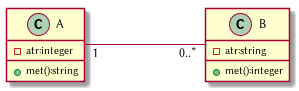
\includegraphics[width=.4\linewidth]{diagramas_clases/diagrama_clase_ejemplo_1.png}
	\caption{Diagrama de Clases - Modelo ejemplo 1}
	\label{fig:dc_mod_ej_1}
\end{figure}

Una vez el modelo esté hecho, es relativamente sencillo trasnmitirlo a su
equivalente en formato de texto. A continuación el modelo escrito en lenguaje
Director.

\lstinputlisting[caption={Director - Modelo para la \texttt{Figura
\ref{fig:dc_mod_ej_1}}}, numbers=left]{modelos-drt/ej1/ej1.txt}

Las cuestiones a tener en cuenta a la hora de analizar el resultado obtenido en
la generación del código a partir del modelo son las siguientes:
\begin{itemize}
	\item \texttt{Fragmento \ref{fig:dc_mod_ej_1}/Linea 1}: aquí se determina que
		el lenguaje de salida será Python.
	\item \texttt{Fragmento \ref{fig:dc_mod_ej_1}/Linea 4}: esta permite al
		programa conocer la estructura de salida del código, en este caso se va a
		presentar el código (con todas las clases involucradas) en un solo archivo,
		mas adelante se ve otro ejemplo utilizando Java, en donde es obligatorio
		definir unicamente una\footnote{Siempre y cuando no se esté hablando de una
		clase embebida} clase por archivo.
\end{itemize}

Éste modelo descrito en lenguaje Director dará como resultado el código
presentado en el \texttt{Fragmento \ref{lst:pyej1}}:

\lstinputlisting[caption={Python - Ejemplo 1, Código generado}, numbers=left,
language=Python, label=lst:pyej1]{modelos-drt/ej1/Ejemplo/Ejemplo.py}

Otra cuestión que puede resultar interesante en el código generado
anteriormente es, \textit{¿Donde se ve la relación? ¿Qué nombre se designa a la
relación si no se establece ningún rol explícitamente en el modelo? (lo que
está sucediendo en dicho código)}.

La relación de las clases se representan mediante el uso de atributos, y la
aparicion de los mismos dependerá de la direccionalidad de la relación
\cites{seidl2012}{pooii2017}, en este caso, el diagrama muestra que la relación es
\textit{bidireccional}, por lo tanto ambas clases deben tener atributos que
representen a la otra, con respecto al nombre a utilizar si no se provee el
\textit{rol} que cada clase cumple en la relación, Director genera un nombre
generico que contiene a las dos clases en cuestion, en este caso genera
\texttt{rel\_A\_B} y \texttt{rel\_B\_A}.

\section{Ejemplo 2}
Como segundo ejemplo, se puede plantear algo que se ve a menudo a la hora de
trabajar con sistemas de información, se mantendrá este ejemplo simple para así
poder abarcar el resultado de la mejor manera.

\textbf{Consigna:}
\begin{displayquote}
	Considerese un módulo de sistema que se encarga de la facturación de
	una entidad, en donde una factura tiene información propia como \textit{número
	y tipo de factura}, en donde el tipo puede tener información propia como una
	\textit{descripción e información impositiva} y además, cuenta con una lista
	de productos (el detalle de la factura).
\end{displayquote}

Una posibilidad para un diagrama de clases que permita modelar este
comportamiento es el clásico \textit{cabecera-detalle}, descrito a
continuación:

\begin{figure}[H]
	\centering
	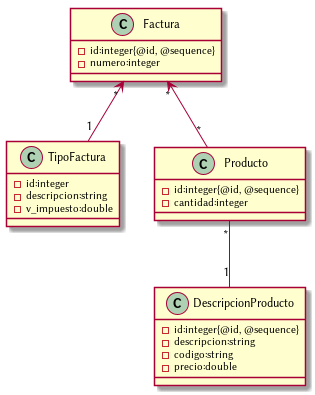
\includegraphics[width=.4\linewidth]{diagramas_clases/diagrama_clase_ejemplo_2.png}
	\caption{Diagrama de Clases - Modelo ejemplo 2}
	\label{fig:dc_mod_ej_2}
\end{figure}

Teniendo este diagama de clases, se puede transferir la informacion a un modelo
Director, éste quedaría de la siguiente manera:

\lstinputlisting[language=Director, caption={Director - Modelo equivalente a la
\texttt{Figura \ref{fig:dc_mod_ej_2}}}, label=lstdrt2,
numbers=left]{modelos-drt/ej2/ej2.txt}

Con éste modelo, el lenguaje, generaría las cuatro clases que se definieron
para el mismo, más una que seria el punto de inicio para el programa Java, éste
último se toma como el nombre del proyecto.

Las clases que se generan se presentan a continuación:

\lstinputlisting[language=Java, caption={Java - Ejemplo 2, Clase generada
\texttt{Facturacion.java}}, label=ej2facturacion,
numbers=left]{modelos-drt/ej2/Facturacion/Facturacion.java}

\lstinputlisting[language=Java, caption={Java - Ejemplo 2, Clase generada
\texttt{TipoFactura.java}}, label=ej2tipofactura,
numbers=left]{modelos-drt/ej2/Facturacion/TipoFactura.java}

\lstinputlisting[language=Java, caption={Java - Ejemplo 2, Clase generada
\texttt{Producto.java}}, label=ej2producto,
numbers=left]{modelos-drt/ej2/Facturacion/Producto.java}

\lstinputlisting[language=Java, caption={Java - Ejemplo 2, Clase generada
\texttt{DescripcionProducto.java}}, label=ej2descripcionproducto,
numbers=left]{modelos-drt/ej2/Facturacion/DescripcionProducto.java}

\lstinputlisting[language=Java, caption={Java - Ejemplo 2, Clase generada
\texttt{Factura.java}}, label=ej2factura,
numbers=left]{modelos-drt/ej2/Facturacion/Factura.java}

\section{Ejemplo 3}
\label{sec:ej3}
En esta sección se abordará un ejemplo más extenso que los vistos anteriormente,
aqui, se presenta un escenario real, utilizado como un trabajo integrador para
la cátedra Programación Orientada a Objetos I, en el año 2017, dicha consigna
fue confeccionada por el Lic. Claudio O. Biale.\\

\textbf{Consigna:}
\begin{displayquote}
Una empresa de reparación de artículos, por ejemplo, hardware de computadoras
desea implementar un sistema de gestión de reclamos.

El sistema debe soportar el ingreso de reclamos, la asignación de recursos para
la reparacióñ de los artículos y el seguimiento de las reparaciones.

El sistema deberá registrar para cada reclamo un número, la descripción del
problema, el tipo de artículo a reparar, la fecha en la que fue ingresado al
sistema y la fecha estimada de entrega. De los tipos de artículos interesa
registrar un código (que lo identifica) y un nombre.

Los reclamos serán reparados por los técnicos de la empresa, los cuales deberan
estar registrados en el sistema. De cada técnico interesa saber su documento
único, nombres, apellidos y los tipos de articulos sobre los que está
capacitado para trabajar. Un técnico puede trabajar como empleado mensual o
jornalero. En caso de ser jornalero interesa conocer la tarifa por hora que se
le paga, mientras que para un empleado mensual interesa conocer el sueldo
mensual que percibe.

Para realizar una reparación, se planifica de entre el conjunto de tareas
definidas en el sistema, una secuencia de tareas que son las que los técnicos
deberán de realizar para concluir la reparación. De las tareas interesa su
código único, nombre, descripción y tipos de artículos a los que aplica. Cada
tarea de una reparación será efectuada por un técnico de la empresa capacitado
en el tipo de artículo a reparar.

Es de interés para la empresa llevar un registro del tiempo invertido por el
técnico en cada tarea realizada. Por ello, será necesario registrar en el
sistema la cantidad de horas dedicadas y el dia que se realizó la tarea. Si la
misma es efectuada en más de un día, interesa saber cuantas horas le dedicó
para cada fecha. Se debe indicar cuando se finaliza la tarea.
\end{displayquote}

Aquí se presenta el diagrama de clases que modela un posible resultado para el
problema en cuestión.

\begin{figure}[H]
	\centering
	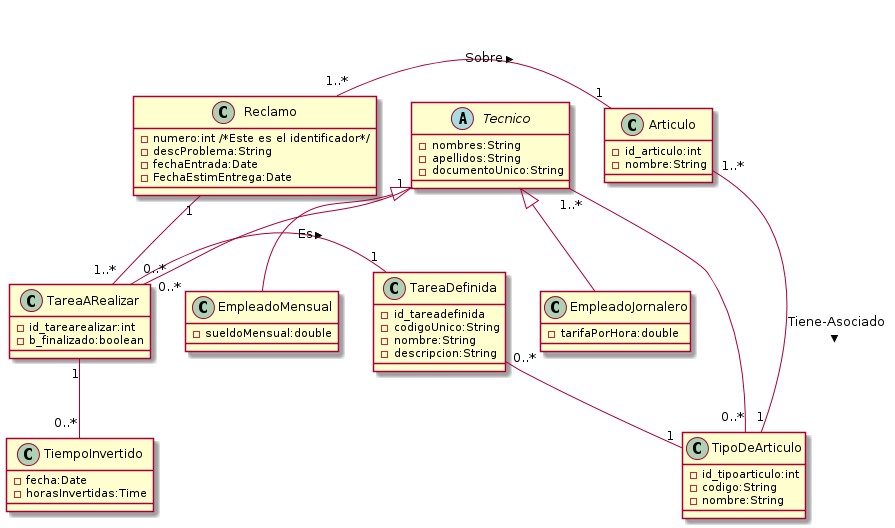
\includegraphics[width=.6\linewidth]{diagramas_clases/diagrama_clase_ejemplo_3.png}
	\caption{Diagrama de Clases - Modelo ejemplo 3}
	\label{fig:dc_mod_ej_3}
\end{figure}

Y luego de pasarlo a un modelo Director se termina teniendo lo siguiente:

\lstinputlisting[language=Director, caption={Director - Modelo equivalente a la
\texttt{Figura \ref{fig:dc_mod_ej_3}}}, label=lstdrt3, numbers=left]
{modelos-drt/ej3/ej3.txt}

A partir del modelo, Director pasará a generar las nueve clases descritas más
una que será el punto de inicio (por el hecho de que la salida está configurada
para ser Java).

\lstinputlisting[language=Java, caption={Java - Ejemplo 3, Clase generada
\texttt{Reparaciones.java}}, label=ej2factura,
numbers=left]{modelos-drt/ej3/Reparaciones/Reparaciones.java}

\lstinputlisting[language=Java, caption={Java - Ejemplo 3, Clase generada
\texttt{Reclamo.java}}, label=ej2facturacion,
numbers=left]{modelos-drt/ej3/Reparaciones/Reclamo.java}

\lstinputlisting[language=Java, caption={Java - Ejemplo 3, Clase generada
\texttt{Articulo.java}}, label=ej2tipofactura,
numbers=left]{modelos-drt/ej3/Reparaciones/Articulo.java}

\lstinputlisting[language=Java, caption={Java - Ejemplo 3, Clase generada
\texttt{TareaDefinida.java}}, label=ej2producto,
numbers=left]{modelos-drt/ej3/Reparaciones/TareaDefinida.java}

\lstinputlisting[language=Java, caption={Java - Ejemplo 3, Clase generada
\texttt{TipoDeArticulo.java}}, label=ej2descripcionproducto,
numbers=left]{modelos-drt/ej3/Reparaciones/TipoDeArticulo.java}

\lstinputlisting[language=Java, caption={Java - Ejemplo 3, Clase generada
\texttt{TareaARealizar.java}}, label=ej2factura,
numbers=left]{modelos-drt/ej3/Reparaciones/TareaARealizar.java}

\lstinputlisting[language=Java, caption={Java - Ejemplo 3, Clase generada
\texttt{TiempoInvertido.java}}, label=ej2facturacion,
numbers=left]{modelos-drt/ej3/Reparaciones/TiempoInvertido.java}

\lstinputlisting[language=Java, caption={Java - Ejemplo 3, Clase generada
\texttt{Tecnico.java}}, label=ej2tipofactura,
numbers=left]{modelos-drt/ej3/Reparaciones/Tecnico.java}

\lstinputlisting[language=Java, caption={Java - Ejemplo 3, Clase generada
\texttt{EmpleadoMensual.java}}, label=ej2producto,
numbers=left]{modelos-drt/ej3/Reparaciones/EmpleadoMensual.java}

\lstinputlisting[language=Java, caption={Java - Ejemplo 3, Clase generada
\texttt{EmpleadoJornalero.java}}, label=ej2descripcionproducto,
numbers=left]{modelos-drt/ej3/Reparaciones/EmpleadoJornalero.java}
